\documentclass[12pt,a4paper]{article}
\usepackage[T1]{fontenc}
\usepackage[utf8]{inputenc}
\usepackage[polish]{babel}
\usepackage[nofoot,hdivide={2cm,*,2cm},vdivide={2cm,*,2cm}]{geometry}
\usepackage{indentfirst}
\usepackage{menukeys}
\usepackage{listings}
\usepackage{graphicx}
\usepackage{pdfpages}
\usepackage{hyperref}
\pagenumbering{gobble}

\usepackage{hyperref}
\hypersetup{
    colorlinks=true,
    linkcolor=black,
    urlcolor=cyan,
}

\graphicspath{ {./img/} }

\begin{document}
\author{Michał Mikołajczyk}
\title{
	\textbf{Dokumentacja gry MineSweeper}\\
	\large Projekt w ramach Programowania Obiektowego\\
	\large Uniwersytet Wrocławski\\
	\large Język C++
	}

\maketitle

\tableofcontents
\newpage

\section{Zasady gry}
Ten projekt jest klonem klasycznego \textit{Minesweepera} znanego z wielu systemów operacyjnych Microsoftu. W tej wersji oprócz pustych pól oraz bomb, generowane są również bloki z flarami, które po naciśnięciu automatycznie odkrywają pola dookoła nich oraz oznaczą pobliskie miny flagą.
\subsection{Plansza}
Polem gry jest plansza zbudowana z pojedynczych bloków. Każdy blok na planszy jest jednym z trzech typów:
\begin{itemize}
\item \textbf{Blok pusty}
\item \textbf{Mina}
\item \textbf{Flara}
\end{itemize}

\subsection{Cele i mechanika gry}
\begin{itemize}
\item Gracz może oznaczyć dowolny blok flagą, co zapobiega odkryciu tego bloku.
\item Odkrycie pustego bloku, który nie ma w pobliżu żadnych min powoduje odkrycie wszystkich jego sąsiadów.
\item Jeżeli ilość sąsiadów oznaczonych flagą bloku pustego jest równa ilości pobliskich min (ukazanej na tym bloku), to możemy nacisnąć na ten blok pusty co spowoduje odkrycie wszystkich nieoznaczonych sąsiadów tego bloku. (w tym min, jeżeli bloki nie zostały oznaczone poprawnie!)
\item Naciśnięcie na odkrytą flarę powoduje oznaczenie pobliskich min oraz odkrycie sąsiadujących bloków pustych.
\item Flary stanowią 3\% bloków na planszy.
\item Miny stanowią 16\% bloków na poziomie \textit{easy} + 1\% więcej na każdym kolejnym poziomie trudności -- kończąc na 20\% przy poziomie \textit{custom - expert}.
\item Gra kończy się przegraną przy odkryciu dowolnej miny.
\item Gra kończy się wygraną jeżeli jedyne ukryte bloki na planszy to miny.
\end{itemize}

\subsection{Sterowanie}
\begin{itemize}
\item \keys{LMB} (Lewy Przycisk Myszy) - odkrycie miny.
\item \keys{RMB} (Prawy Przycisk Myszy) - oznaczenie bloku flagą.
\item \keys{R} - szybki restart.
\end{itemize}

\newpage

\subsection{Interfejs i ustawienia}
\begin{itemize}
\item Na samej górze okna widoczne są statystyki obecnej gry: czas, oznaczone miny oraz ilość flar dostępnych na tej planszy.
\item W prawym górnym rogu znajdują się przyciski resetu gry oraz ustawień.
\item Na ekranie ustawień możemy zmienić kolor bloków oraz poziom trudności.
\item Po wybraniu poziomu \textit{custom - expert}, w prawej stronie okna ustawień pojawią się pola, w które można wpisać własny rozmiar planszy. Maksymalny rozmiar to 100x100.
\end{itemize}
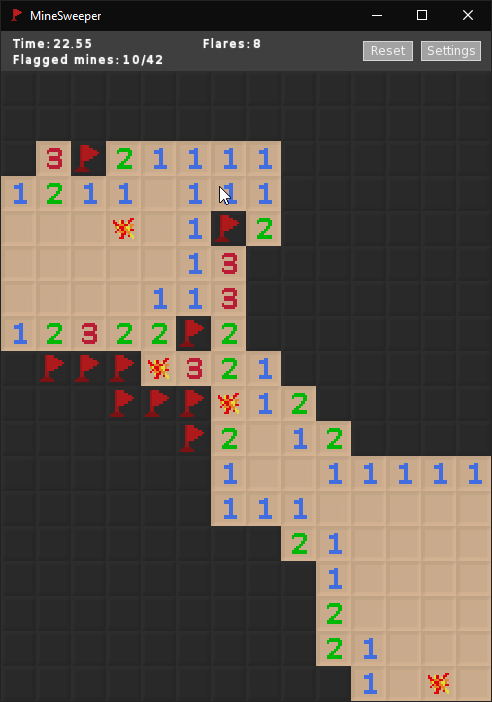
\includegraphics[scale=0.45]{game}
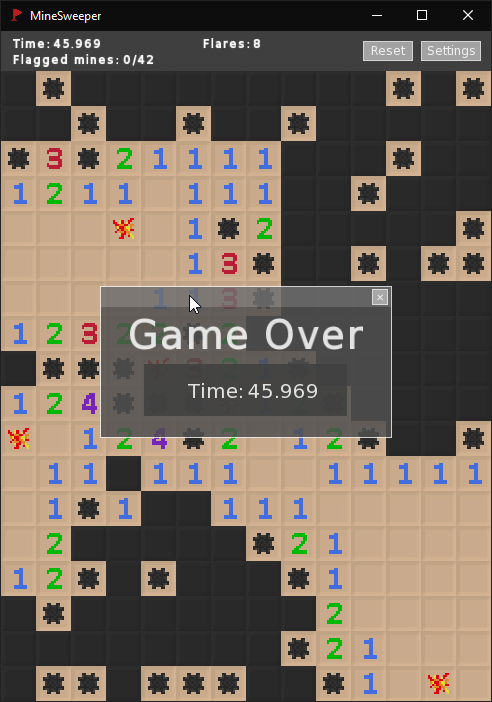
\includegraphics[scale=0.45]{gameOver}

\includegraphics[scale=0.45]{settings}
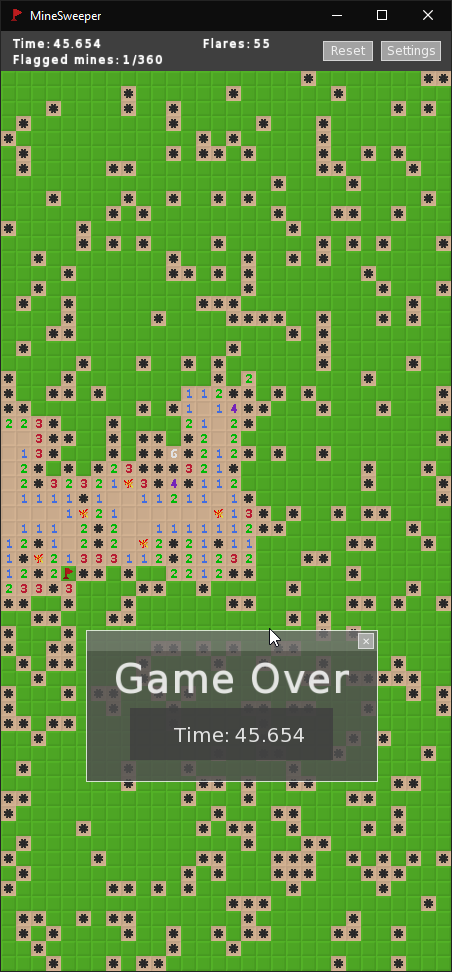
\includegraphics[scale=0.45]{g3}
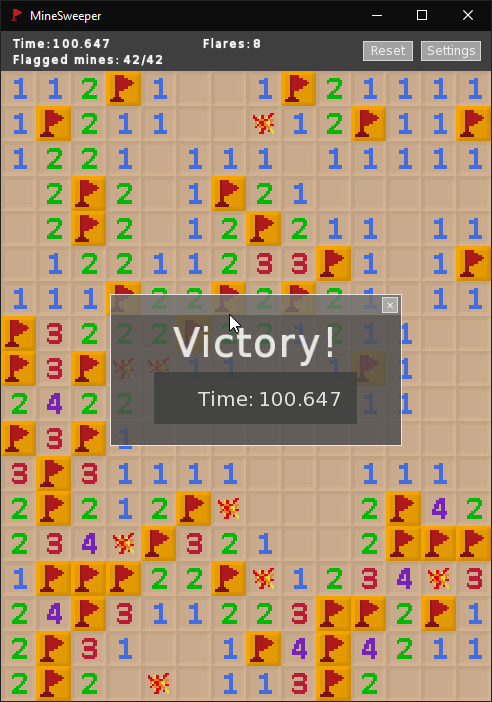
\includegraphics[scale=0.45]{g2}
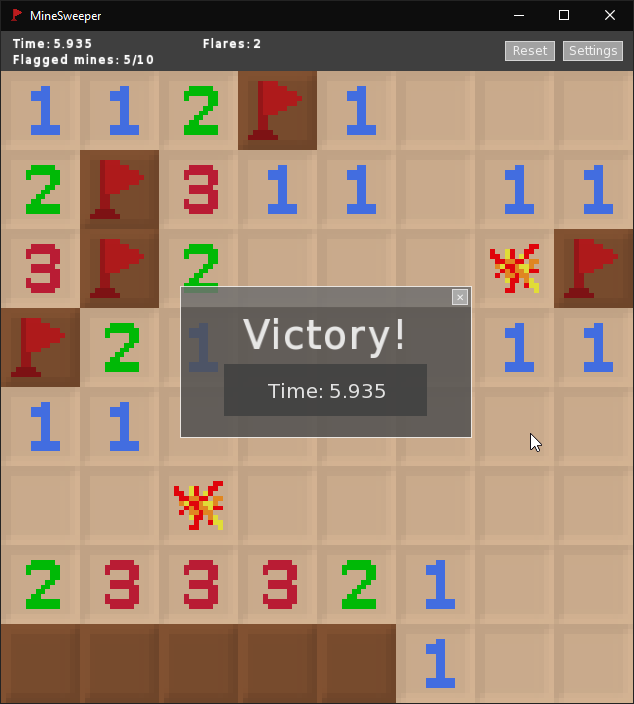
\includegraphics[scale=0.36]{g1}




\newpage
\section{Podział na klasy}
\subsection{Diagram UML}
Diagram został wygenerowany za pomocą programu \href{https://www.bouml.fr/}{Bouml}.\\ \
\begin{figure}
 \centering 
 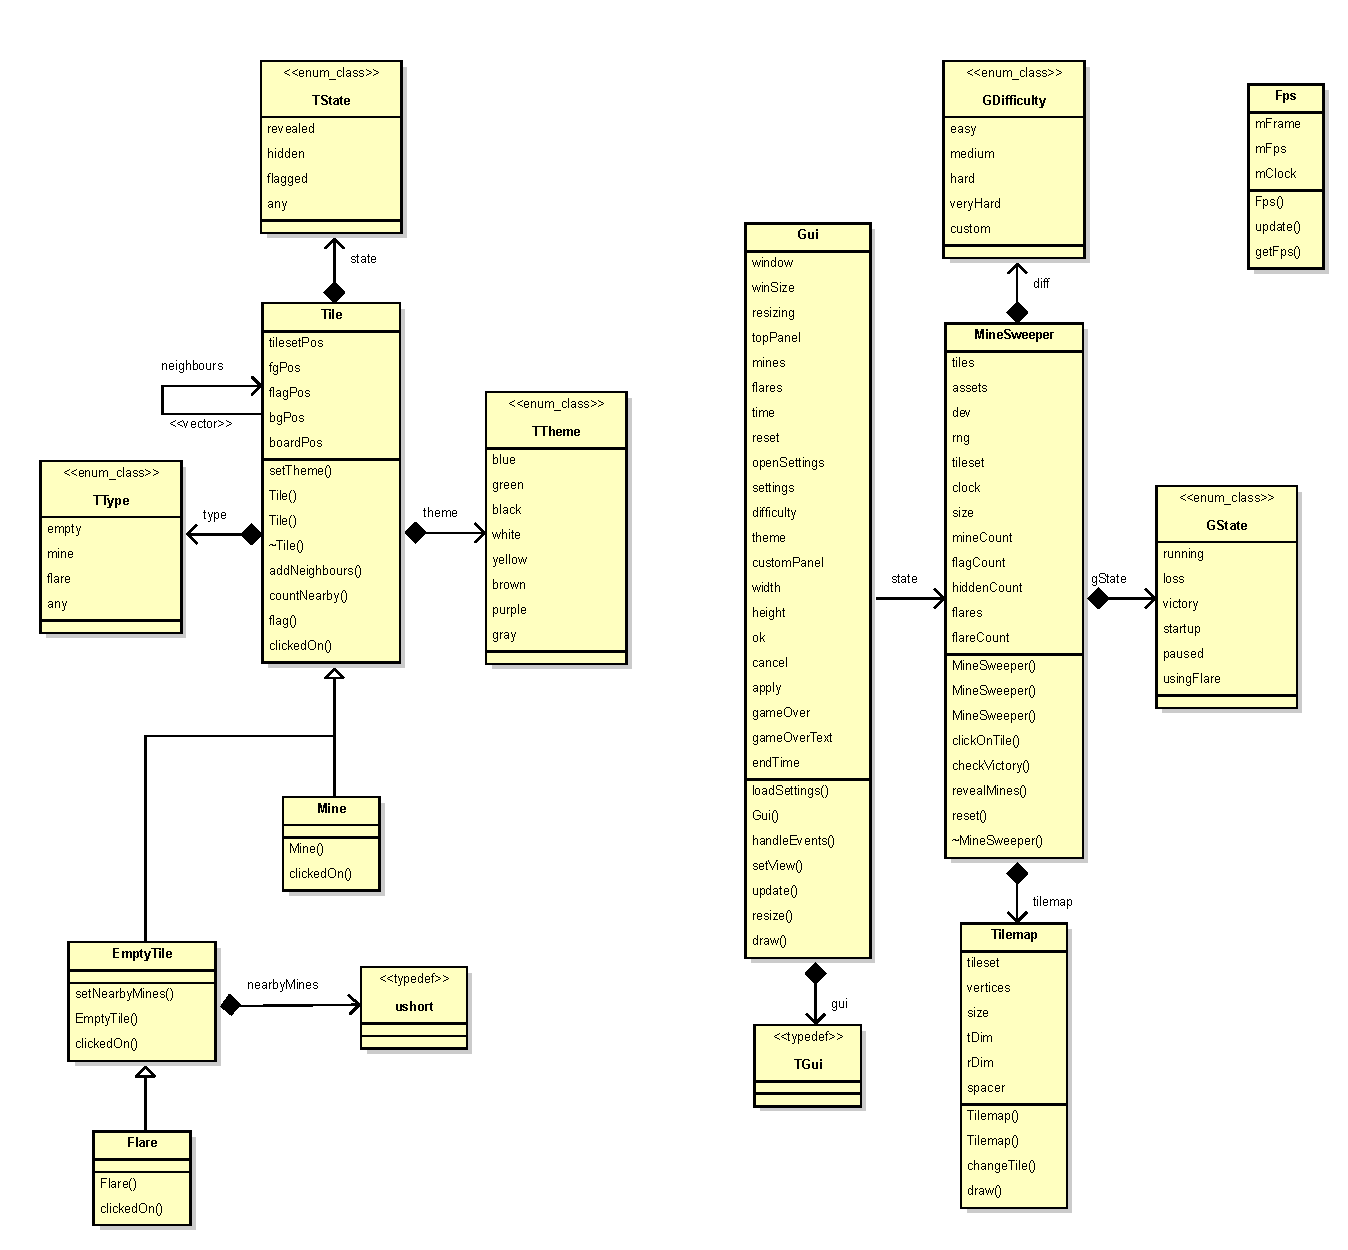
\includepdf[pages=1,offset=0 -40,scale=0.9]{diagram.pdf}
\end{figure}

\newpage

\subsection{Lista klas i ich funkcje}
\begin{itemize}
\item \textbf{MineSweeper} - główna klasa projektu. Zawiera informacje o stanie gry oraz tekstury planszy i bloków.

\item \textbf{Tilemap} - klasa dziedzicząca po klasie abstrakcyjnej sf::Drawable z biblioteki SFML. Jej zadaniem jest tworzenie i modyfikacja siatki wierzchołków, na której wyświetlane są tekstury bloków. Dzięki tej klasie gra działa dużo szybciej i jest w stanie wyświetlać dziesiątki tysięcy bloków na raz, ponieważ zamiast wywoływać funkcję draw() dla każdego bloku, możemy użyć tylko jednej, rysującej teksturę stworzoną z siatki przechowywanej w obiekcie Tilemap.

\item \textbf{Tile} - klasa abstrakcyjna bloku. Zawiera funkcje pozwalające na przypisanie jej sąsiadujących z nią bloków, oznaczenie bloku flagą, zliczenie sąsiadów o danym stanie i typie oraz metodę czysto wirtualną -- \textit{clickedOn()}, która jest wywoływana gdy gracz naciska na blok. Metoda ta jest nadpisywana przez każdą klasę dziedziczącą po \textit{Tile}.

\item \textbf{Mine} - klasa dziedzicząca po \textit{Tile} reprezentująca minę.

\item \textbf{EmptyTile} - klasa dziedzicząca po \textit{Tile} reprezentująca pusty blok. Zawiera atrybut \textit{nearbyMines} oraz funkcję \textit{setNearbyMines()} liczącą pobliskie miny.
\item \textbf{Flare} - klasa dziedzicząca po \textit{EmptyTile} reprezentująca flarę.

\item \textbf{Gui} - klasa będąca wrapperem obiektu klasy tgui::Gui z biblioteki TGUI. Odpowiada za wczytywanie interfejsu z pliku, za podpięcie wskaźników na jego elementy oraz za jego aktualizację.

\item \textbf{Klasy enumeracyjne} - te klasy odpowiadają za przypisanie wartości nazwom:
\begin{itemize}
\item \textbf{TState} - stan bloku,
\item \textbf{TType} - typ bloku,
\item \textbf{GState} - stan gry,
\item \textbf{GDifficulty} - poziom trudności.
\end{itemize}

\item \textbf{Fps} - mała klasa odpowiadająca za zliczanie ilości klatek na sekundę. W końcowej wersji gry nie jest ona wykorzystywana.

\end{itemize}

\newpage

\section{Wymagania}
\subsection{System operacyjny}
Gra została napisana dla systemów 64 bitowych Microsoft Windows.

\subsection{Zasoby}
Co najmniej 100MB wolnej pamięci RAM. Podczas testowania, przy maksymalnym rozmiarze planszy (100x100), program zajmował ok. 58MB w pamięci w wersji Debug oraz ok. 42MB w wersji Release.

\subsection{Biblioteki linkowane dynamicznie}
\begin{itemize}
\item \Large \textbf{SFML}\\
Simple and Fast Multimedia Library\\
\url{https://www.sfml-dev.org/}
\item \Large \textbf{TGUI\_TTF}\\
Texus' Graphical User Interface\\
\url{https://tgui.eu/}
\end{itemize}

\subsection{Środowisko programistyczne}
Ten projekt został napisany przy pomocy środowiska Visual Studio 2017.
Program jest kompilowany przez Visual Studio automatycznie, przy użyciu CMake.
\end{document}